\section{Initial Conditions}

The influence of the initial conditions on the motion of the leaf can be investigated. The initial conditions explain the velocity, angle and angular velocity at the point when the leaf is set in motion. The initial position will not change the trajectory of the leaf since the space in which the leaf falls is assumed the same in all places, therefore this initial condition will not be considered. The influence can be measured % better word than measured
by comparing the trajectory and velocity of the leaf in the long term with those discussed in section \ref{sec:motion}. To ensure the comparison is relevant the same parameter values will be used that is $f=100, l=1, \rho = 0.1, g = 9.81$. The value of the friction perpendicular to leaf will then be varied to take the same values as in section \ref{sec:motion}, $k_{\perp}$=$4.84,4.9,9.75,12,50$.
\\
\\
The initial angle of the leaf must fall in the limits $-\frac{\pi}{2}<\theta<\frac{\pi}{2}$. The initial angle will be investigated for $-1.5\leq \theta \leq1.5$ in steps of 0.3. 
\\
\\
For $k_{\perp}=4.84$ and $k_{\perp}=4.9$ the initial angle has no influence on the behaviour of the leaf. However for some angles it will change the direction the leaf falls. For $k_{\perp}=9.75$ the initial angle has no noticeable influence, the leaf fell with no pattern when the initial angle $\theta=1$, and this was repeated for all other initial angles. When $k_{\perp}=12$ the leaf showed the same swaying motion in the long term. However for values of $\theta$ with a larger magnitude the leaf initially fell with a more random motion such as that seen for $k_{\perp}=9.75$. The trajectory and velocity of a leaf with initial conditions $u=v=\omega =0$ and $\theta=0.6$ is shown in Figure \ref{fig:kper12theta0_6}. The parameters were set at $f=100, l=1, \rho = 0.1, g = 9.81, k_{\perp} = 12$.

\begin{figure}[H]
\centering
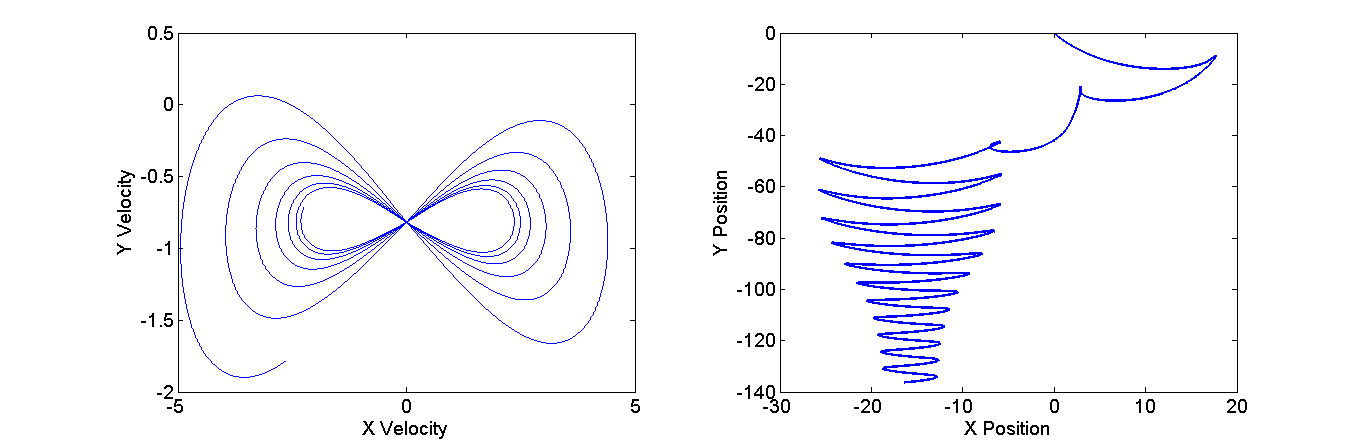
\includegraphics[width=0.7\textwidth]{IA-1_2_kper12.png}
\caption{\label{fig:kper12theta0_6}(Left)Plot showing the velocity in the x and y direction after transients have decayed. (Right) Plot showing the position of the leaf in the x and y direction.
}
\end{figure}


For $k_{\perp}=50$ the initial angle does have some influence on the motion of the leaf. A larger magnitude of the initial angle causes the leaf to fall faster initially so it travels further in the vertical direction and drifts further in the x direction. However, all solutions eventually reach what appears to be an equilibrium falling vertically with $\theta=0$. 
\\
\\
The initial angular velocity of the leaf can be investigated in a similar manner by varying the initial value of $\omega$ instead of $\theta$. The initial angular velocity will be investigated for $\omega$ between -10 and 10 in steps of 2. The initial angle will be returned to $\theta=1$ for this investigation. 
\\
\\
For $k_{\perp}=4.84$ and $k_{\perp}=4.9$  the initial angular velocity had a similar influence to the initial angle. It did not change the behaviour of the leaf, it only changed the direction of the regular falling motion. For $k_{\perp}=9.75$ the leaf showed the same falling pattern for all values of $\omega$ as seen in Section \ref{sec:motion}. For $k_{\perp}=12$ the motion of the leaf is similar to that shown for $k_{\perp}=9.75$, before settling to the swaying motion previously seen for $k_{\perp}=12$. This is shown in Figure \ref{fig:kper12Omega0_2} where the initial value of $\omega=2$. As the initial value of $\omega$ moves further from zero the motion settles to a swaying motion sooner as shown in Figure \ref{fig:kper12Omega0_10} where the initial value of $\omega=10$. The parameters are set at $f=100, l=1, \rho = 0.1, g = 9.81, k_{\perp} = 12$. 

\begin{figure}[H]
\centering
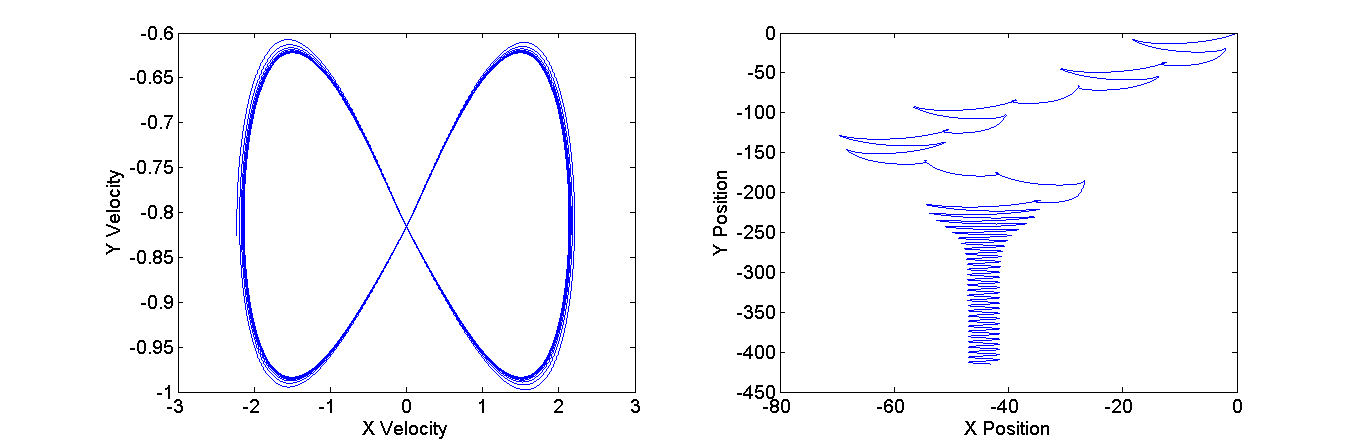
\includegraphics[width=0.7\textwidth]{IO_2_kper_12.png}
\caption{\label{fig:kper12Omega0_2}(Left)Plot showing the velocity in the x and y direction after transients have decayed. (Right) Plot showing the position of the leaf in the x and y direction.
}
\end{figure}

\begin{figure}[H]
\centering
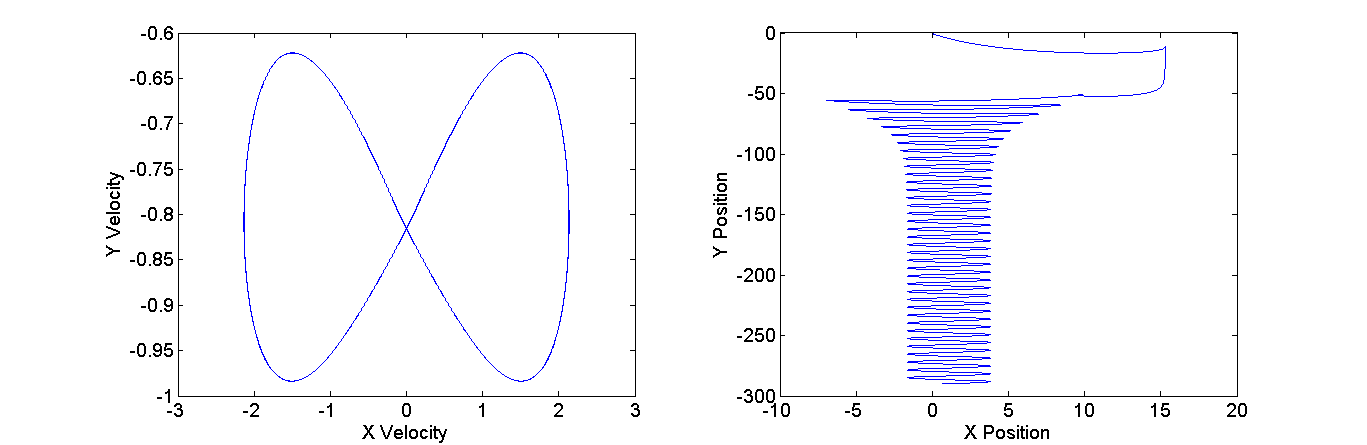
\includegraphics[width=0.7\textwidth]{IO_10_kper_12.png}
\caption{\label{fig:kper12Omega0_10}(Left)Plot showing the velocity in the x and y direction after transients have decayed. (Right) Plot showing the position of the leaf in the x and y direction.
}
\end{figure}

For $k_{\perp}=50$ the initial angular velocity had no noticeable influence on the motion of the leaf. The leaf drifted to the left before falling vertically as seen in Section \ref{sec:motion}.
\\
\\
The initial velocity of the leaf can also be considered, the velocities in the x and y directions will be considered separately. The initial velocities considered will again range from -10 to 10 in steps of 2. 
\\
\\
The initial velocity in the x-direction has no influence on the behaviour of the leaf for $k_{\perp}=4.84$ and $k_{\perp}=4.9$. The initial velocity only changed the direction in which the leaf fell. For $k_{\perp}=9.75$ the initial velocity changed the behaviour of the fall. The leaf still fell in a swaying motion followed by more random motion, however, the swaying motion lasted for a greater distance than it did for other initial conditions.%This needs to be rewritten.
This is shown in Figure \ref{fig:kper9.75U0_6} where the initial velocity in the x direction is 6.

\begin{figure}[H]
\centering
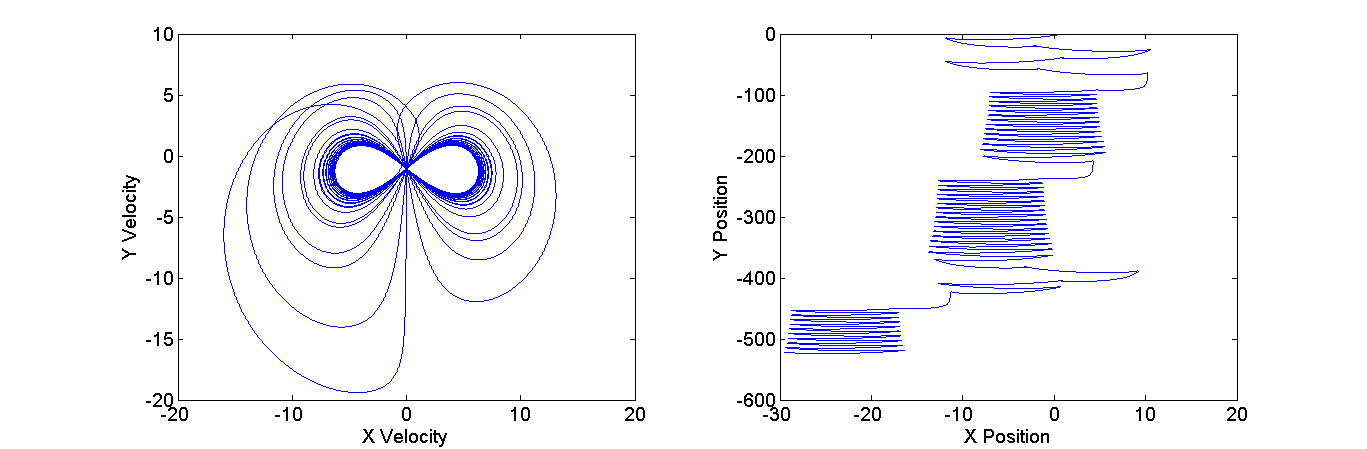
\includegraphics[width=0.7\textwidth]{IU_6_kper_9_75.png}
\caption{\label{fig:kper9.75U0_6}(Left)Plot showing the velocity in the x and y direction after transients have decayed. (Right) Plot showing the position of the leaf in the x and y direction.
}
\end{figure}

As $k_{\perp}$ is increased further to 12 the leaf shows random movement before settling to the expected swaying motion for initial values of u not equal to zero. For $k_{\perp}=50$ the initial velocity in the x direction had no influence on the behaviour of the leaf. The leaf slowly fell to the left before settling to a vertical fall. 
\\
\\
As with the initial velocity in the x direction, the initial velocity in the y direction does not influence the behaviour of the leaf it only changes the direction of the fall for $k_{\perp}=4.84$ and $k_{\perp}=4.9$.
For $k_{\perp}=9.75$ the initial velocity in the y direction does not influence the motion of the leaf. The leaf still falls with periods of swaying motion followed by random motion. %Find a better phrase for 'random motion' 
For $k_{\perp}=12$ the motion is not influenced by the initial velocity, the leaf falls to the ground with a swaying motion for all values in the initial velocity range. Similarly for $k_{\perp}=50$ the motion is not influenced by the initial velocity, the leaf drifts to the left before falling vertically for all initial velocities in the range.
\\
\\
The initial conditions did influence the behaviour of the falling leaf for some parameter values but largely had no influence in the long term. The only condition that altered the fall in the long term was the initial velocity in the x direction with $k_{\perp}=9.75$. Although the overall pattern of random falling followed by periods of swaying motion was observed the distance covered during the swaying motion was much larger. 
\\
\\